%TODO: add cliffhanger with preview for next time

% Make nice A4 pages for print:
%\usepackage{pgfpages}
%\pgfpagesuselayout{resize to}[a4paper,border shrink=5mm,landscape]

\beamertemplatenavigationsymbolsempty

\setbeamertemplate{bibliography item}[text]

\usepackage[type={CC},modifier={by-sa},version={4.0}]{doclicense}

\usepackage[utf8]{inputenc}
\usepackage{hyperref}
\usepackage{breakurl}
\usepackage{graphicx}
\usepackage{pgfplots}
\usepackage{pgf}
\usepackage{tikz}
\usetikzlibrary{positioning}
\usetikzlibrary{arrows}
\usetikzlibrary{decorations.markings}
\usetikzlibrary{calc}
\usetikzlibrary{matrix}
\usetikzlibrary{shapes}
\usetikzlibrary{decorations.pathmorphing}
\usetikzlibrary{fit}
\usetikzlibrary{backgrounds}
\usetikzlibrary{plotmarks}
\usepackage{stmaryrd}
\usepackage{listings}
\usepackage{pdflscape}
\usepackage{perpage}
\usepackage{appendixnumberbeamer}

%\usepackage[thmmarks,amsmath,amsthm]{ntheorem} % already included in beamer
\usepackage{thm-restate}

\usepackage[sort&compress,numbers]{natbib}  % to be have \citet, \citeauthor, \citeyear

\MakePerPage{footnote}

\tikzstyle{o}=[r,ppBlue]
\tikzstyle{r}=[thick,rectangle,align=center]
\tikzstyle{t}=[r,ppTrans] %,font=\bfseries]
\tikzstyle{dd}=[densely dashed]
\tikzstyle{n}=[r,ppBlue]
\tikzstyle{p}=[r,ppRed]
\tikzstyle{ppRed}  =[draw=red,  fill=  red!20]
\tikzstyle{ppBlue} =[draw=blue, fill= blue!20]
\tikzstyle{ppGreen}=[draw=green,fill=green!20]
\tikzstyle{ppTrans}=[draw=none, fill=none]

\usetheme{Warsaw}

\useoutertheme[subsection=true]{smoothbars}
%\useoutertheme[subsection=false]{miniframes}

\definecolor{bblue}{HTML}{D7DF01}	% yellow-ish actually, for better black/white printing
\definecolor{rred}{HTML}{C0504D}
\definecolor{ggreen}{HTML}{9BBB59}
\definecolor{ppurple}{HTML}{9F4C7C}
\definecolor{lightgray}{rgb}{0.3,0.3,0.3}
\definecolor{lightergray}{rgb}{0.9,0.9,0.9}
\definecolor{UniBlue}{RGB}{83,121,170}

\DeclareTextFontCommand\textintro{\normalfont\bfseries\itshape} % nice!
\newcommand{\intro}[2][]
{%
	\textintro{#2}%
}
\newcommand{\empha}[2][]
{%
	\emph{#2}%
}

%\theoremstyle{plain}
\newcounter{reqcounter}
\newtheorem{requirement}[reqcounter]{Requirement}

%setbeamercolor{structure}{fg=violet}

\makeatletter
\def\th@task{%
    \normalfont % body font
    \setbeamercolor{block title example}{bg=orange,fg=white}
    \setbeamercolor{block body example}{bg=orange!20,fg=black}
    \def\inserttheoremblockenv{exampleblock}
  }
\makeatother

\theoremstyle{task}
\newtheorem{task}{Task}

\newenvironment{assignment}%
{%\setbeamercolor{background canvas}{bg=violet}%
%\setbeamercolor{structure}{fg=cyan!90!black}%
 \setbeamercolor{frametitle}{bg=orange,fg=white}
\begin{frame}}%
{\end{frame}}%

\AtBeginSection[]{
  \begin{frame}
  \vfill
  \centering
  \begin{beamercolorbox}[sep=8pt,center,shadow=true,rounded=true]{title}
    \usebeamerfont{title}\insertsectionhead\par%
  \end{beamercolorbox}
  \tableofcontents
  \vfill
  \end{frame}
}




\pgfplotsset{compat=1.14}
\author{Markus Raab}


\date{20.3.2018}

\begin{document}

\renewcommand{\enquote}[1]{\emph{``#1''}} % Cannot be done earlier

%%%%%%%%%%%%%%%%%%%%%%%%%%%%%%%
\begin{frame}
	\titlepage
	\doclicenseThis
\end{frame}

\begin{frame}
	Lecture is every week Wednesday 09:00 - 11:00.

	\begin{description}
		\item[06.03.2019:] topic, teams
		\item[13.03.2019:] TISS registration, initial PR
		\item[{\color{red}20.03.2019}:] {\color{red}other registrations, Guest Lecture}
		\item[27.03.2019:] first issue done, second assigned, \\ HS: kleiner Schiffbau
		\item[03.04.2019:]
		\item[10.04.2019:] mid-term submission of exercises
		\item[08.05.2019:] (HS?)
		\item[15.05.2019:]
		\item[22.05.2019:]
		\item[29.05.2019:]
		\item[05.06.2019:] final submission of exercises
		\item[12.06.2019:]
		\item[19.06.2019:] last corrections of exercises
		\item[26.06.2019:] exam
	\end{description}
\end{frame}

\begin{frame}
	\frametitle{Popular Topics}
	\vspace{-0.55cm}
	\setlength{\columnsep}{-1.3cm}
	\raggedright
	\begin{multicols}{2}
	\begin{description}
	\item[14] tools
	\item[9] testability
	\item[9] code-generation
	\item[7] context-awareness
	\item[6] specification
	\item[6] misconfiguration
	\item[6] {\color{red} complexity reduction}
	\item[5] validation
	\item[5] points in time % (early detection)
	\item[5] error messages
	\item[5] auto-detection
	\item[4] user interface
	\item[4] introspection
	\item[4] design
	\item[4] cascading
	\item[4] architecture of access
	\item[3] {\color{red} configuration sources}
	\item[3] config-less systems
	\item[2] secure conf
	\item[2] architectural decisions
	\item[1] push vs.\ pull
	\item[1] infrastructure as code
	\item[1] full vs.\ partial
	\item[1] convention over conf %iguration
	\item[1] CI/CD
	\item[0] documentation
	\end{description}
	\end{multicols}
\end{frame}

\begin{frame}
	\frametitle{Talk}
	about anything related to configuration management.
	\begin{itemize}
		\item The duration must be not longer than 20 minutes (shorter is ok, content matters).
		\item It must be about your experience.
		\begin{itemize}
			\item E.g., about the homework you did.
			\item I.e., not only about study of literature.
			\item If you extensively use some tool before, please share your experience.
		\end{itemize}
		\item Two persons per date.
		\item Same topic allowed if persons coordinate their talk.
		\item \textbf{Slides must be in repo \\ (please CC licensed and with source)}
	\end{itemize}
\end{frame}

\begin{assignment}
	\frametitle{Tasks for today}
	(until 20.03.2019 23:59)

	\begin{task}
	Registration for talk, homework, teamwork and
	make sure to say which programming languages you know in STUDENTS.ini.
	\end{task}

	\begin{task}
	Write text in at least one issue.
	\end{task}
\end{assignment}

\begin{assignment}
	\frametitle{Tasks for next week}
	(until 27.03.2019 23:59, hint: to get help submit at least one day earlier)

	\begin{task}
	Description of homework as pull request in private repo.
	(Inside a folder for you, use GitHub name.)
	\end{task}

	\begin{task}
	Description of teamwork (which application, which CM tool) as pull request in private repo.
	(Inside a folder for your team.)
	\end{task}

	\begin{task}
	Fix at least one issue and write some text in at least one other issue.
	\end{task}
\end{assignment}

\begin{frame}
	\hspace*{-1cm}\includegraphics[width=\paperwidth]{dot/topics}
\end{frame}


%%%%%%%%%%%%%%%%%%%%%%%%%%%%%%%%%%%%%%%%%% 
\section{Command-line Arguments}

\subsection{Usage and Popularity}

\begin{frame}
	\frametitle{Is there something else?}
	\begin{itemize}
	\item configuration files are the most researched of all configuration sources~\cite{jin2014configurations}
	\item but it is neither the most used nor most popular~\cite{raab2017challenges}
	\end{itemize}
\end{frame}

\begin{frame}
	\methodQuestion{} \question{Which configuration systems/libraries/APIs have you already used or would like to use in one of your FLOSS project(s)?}
	\begin{itemize}
	\item command-line arguments (\p{92}, $n=222$)
	\item environment variables (\p{79}, $n=218$)
	\item \methodSource{} API \texttt{getenv} is used omnipresently with 2,683 occurrences
	\item configuration files (\p{74}, $n=218$))
	\end{itemize}
\end{frame}


\begin{frame}
	\methodQuestion{} \question{What is your experience with the following configuration systems/libraries/APIs?}
	\begin{itemize}
	\item \texttt{getenv} (\p{10}, $n=198$)
	\item configuration files (\p{6}, $n=190$)
	\item command-line options (\p{4}, $n=210$)
	\item X/Q/GSettings (\p{41}, \p{14}, \p{35})
	\item KConfig (\p{21})
	\item dconf (\p{42})
	\item plist (\p{32})
	\item Windows Registry (\p{69})
	\end{itemize}
\end{frame}

\begin{assignment}
	\begin{task}
	Which configuration source do you use most?
	\end{task}

	\begin{task}
	Possible talk: About one of these sources.
	\end{task}
\end{assignment}

\subsection{Semantics}

\begin{frame}
	\begin{itemize}
	\item passed by main for a new process via \\ (\texttt{int argc, char ** argv})
	\item visible from other processes (e.g., via \texttt{ps aux})
	\item could be passed along to subprocesses but hardly done
	\item need to be parsed by process
	\item portability: differences in parsing
	\item cannot be changed from outside (requires restart, no IPC)
	\end{itemize}
\end{frame}




%%%%%%%%%%%%%%%%%%%%%%%%%%%%%%%%%%%%%%%%%% 
\section{Environment Variables}

\begin{frame}
	\frametitle{Semantics}
	\begin{itemize}
	\item are also per-process (\texttt{/proc/self/environ})
	\item are not visible from other processes
	\item are automatically inherited by subprocesses
	\item need to be parsed by process (\texttt{[extern] char **environ}) but API is provided (\texttt{getenv})
	\item cannot be changed from outside (requires restart or an additional IPC mechanism)
	\end{itemize}
\end{frame}

\begin{assignment}
	\begin{task}
	What is wrong with the code in the book?
	\end{task}
\end{assignment}

\begin{frame}
	\frametitle{getenv}
	\begin{itemize}
	\item is widely standardized, including SVr4, POSIX.1-2001, 4.3BSD, C89, C99~\cite{man2017getenv},
	\item is supported by many programming languages, and
	\item enforces \texttt{key=value} convention.
	\end{itemize}
\end{frame}

\begin{frame}
	\frametitle{Usage}
	\begin{enumerate}
	\item bypassing other configuration accesses (\methodQuestion{} \p{45})
	\item locating configuration files
	\item debugging and testing (\methodQuestion{} \p{55}, \methodSource{} 1,152, i.\,e. \p{43})
	\item sharing configuration settings across applications (\methodQuestion{} \p{53}, \methodSource{} 716, i.\,e. \p{47})
	\item for configuration settings unlikely to be changed by a user (\methodQuestion{} \p{20})
	\item \question{even when it is used inside a loop} (\methodQuestion{} \p{2})
	\end{enumerate}
\end{frame}

\begin{frame}
	\frametitle{Portability}
	\begin{itemize}
	\item no separators for values defined
	\item case sensitivity problems
	\item often many environment variables for the same purpose: TMP, TEMP, or TMPDIR
	\item sometimes one environment variable for different purposes: PATH
	\end{itemize}
\end{frame}



\subsection{Requirements}

\begin{frame}
	How can we deal with the many sources?

	\vspace{1cm}

	\begin{restatable}{requirement}{reqEnvironment}
	A configuration library must support all three popular ways for configuration access:
	configuration files, command-line options, and environment variables.
	\end{restatable}
\end{frame}

\begin{frame}
	\frametitle{Cascading}
	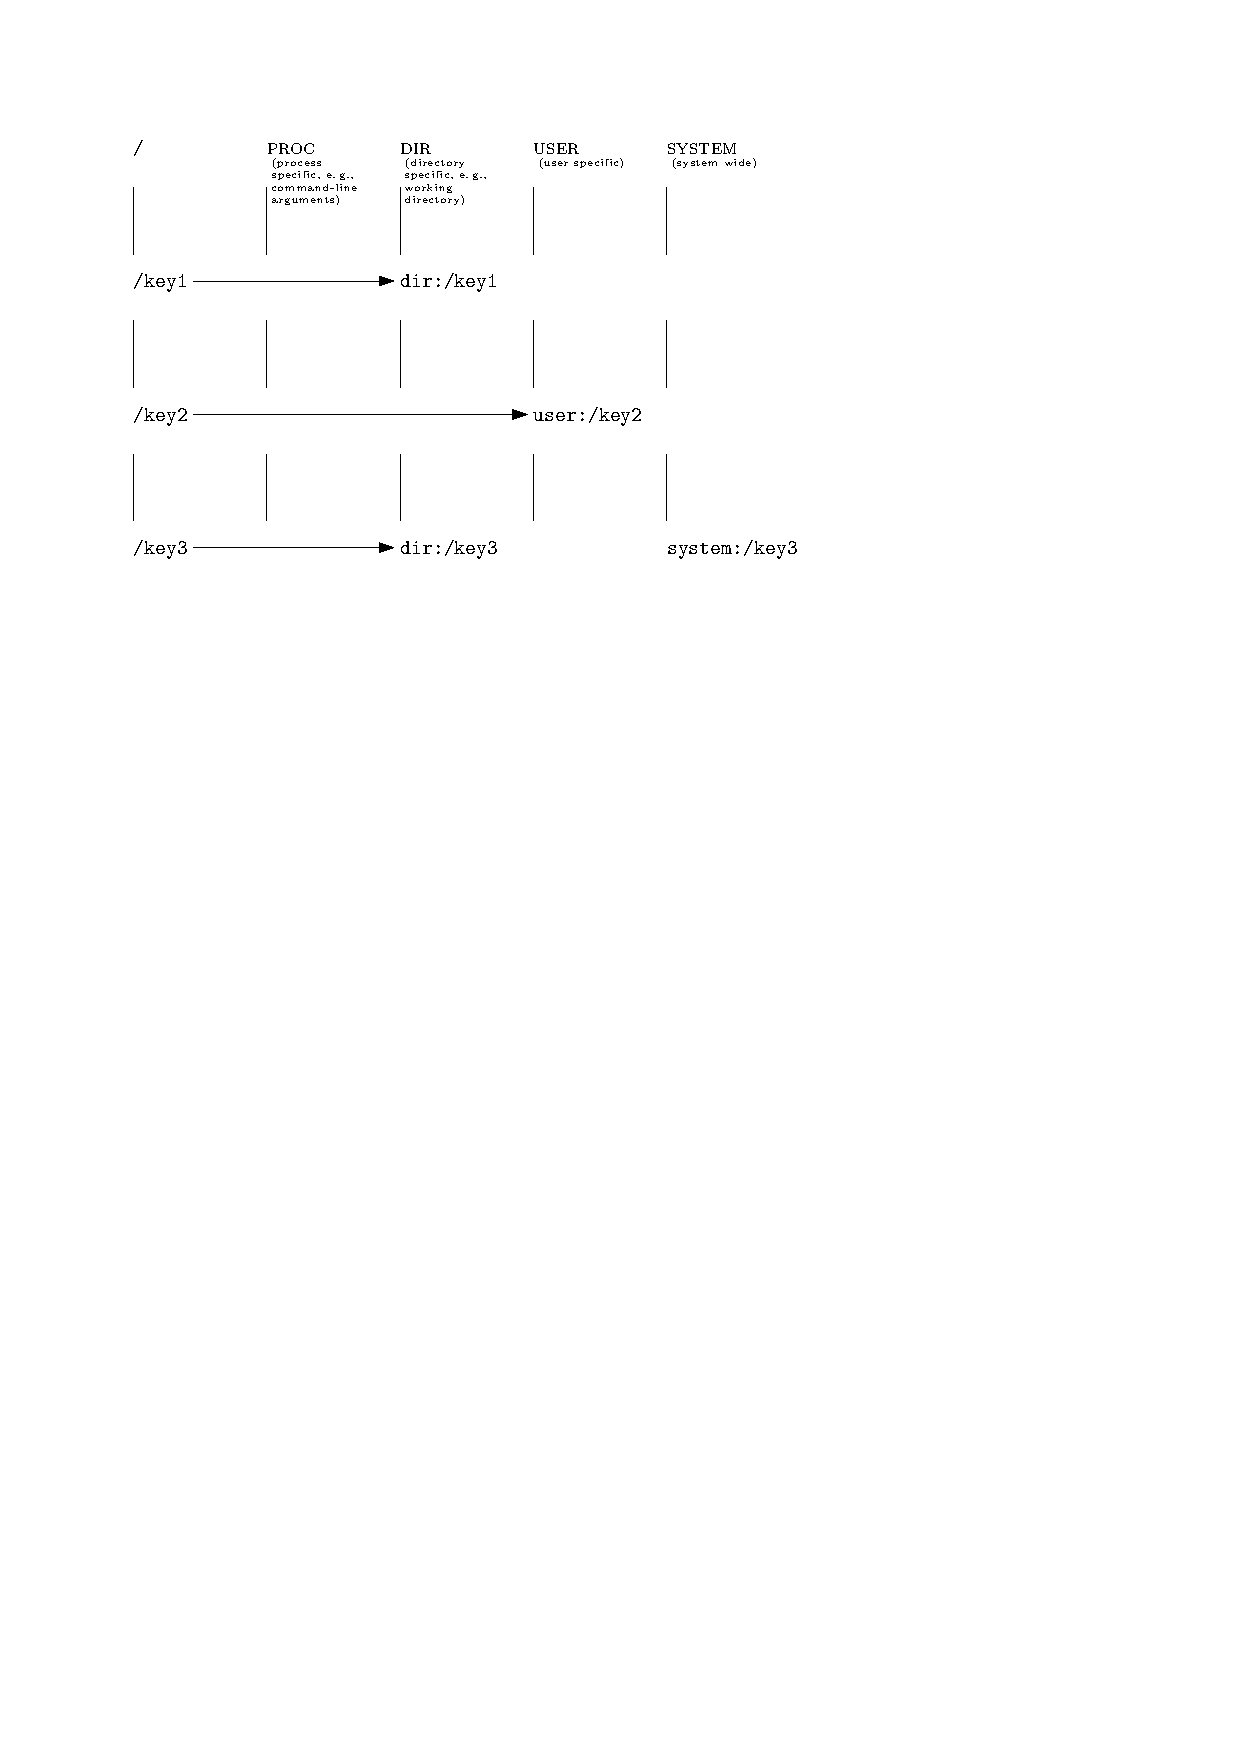
\includegraphics{cascading}
\end{frame}

\begin{assignment}
	\begin{task}
	Discuss the differences of mounting and cascading with your neighbor.
	\end{task}
\end{assignment}


\subsection{Conclusion}

\begin{frame}
	\frametitle{User View}
	\begin{itemize}
	\item command-line for trying out configuration settings
	\item environment variables for configuration settings within a shell
	\item configuration files for persistent configuration settings
	\end{itemize}
\end{frame}

\begin{frame}
	\frametitle{Conclusion}
	\begin{itemize}
	\item three different configuration sources widely used
	\item all three used for different reasons but often for the same configuration settings
	\item many different configuration file formats
	\item abstractions: key-value, mounting, and cascading
	\end{itemize}
\end{frame}






%%%%%%%%%%%%%%%%%%%%%%%%%%%%%%%%%%%%%%%%%% 
\section{Complexity}

\subsection{Trend}

\begin{frame}
	\frametitle{Trend Firefox}
	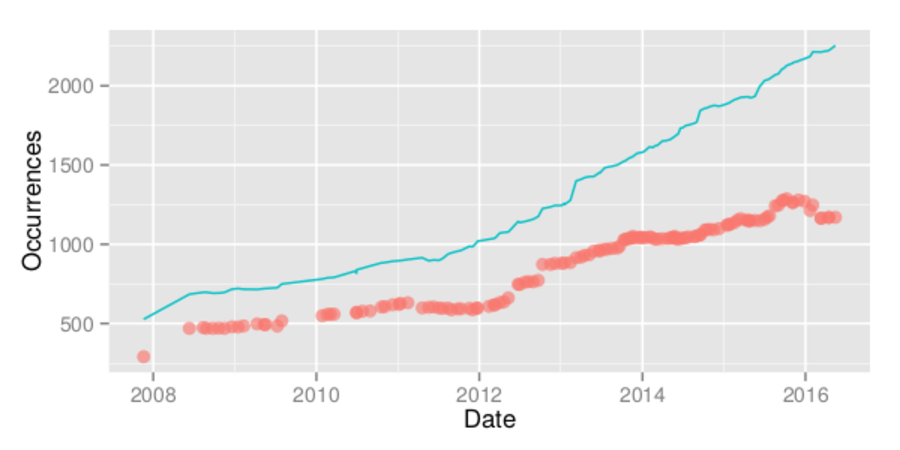
\includegraphics[scale=0.7]{firefox}
\end{frame}

\begin{frame}
	\frametitle{Trend Chromium}
	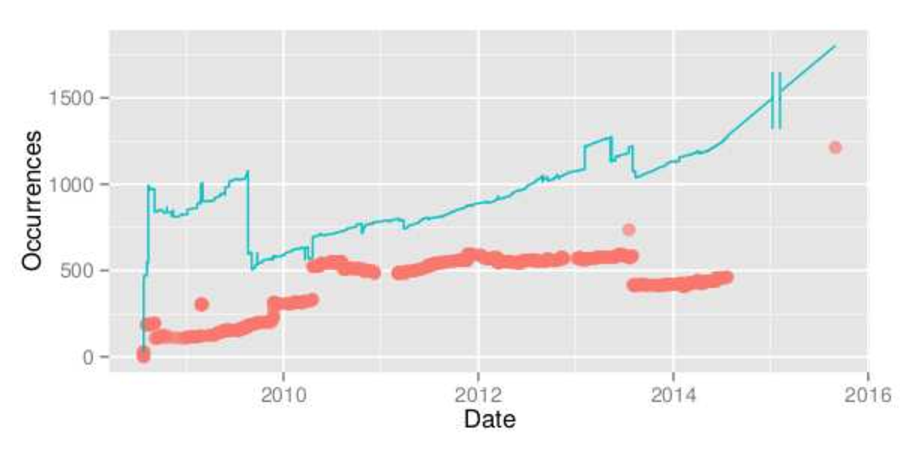
\includegraphics[scale=0.7]{chromium}
\end{frame}

\begin{frame}
	\frametitle{Trend Configuration Files}
	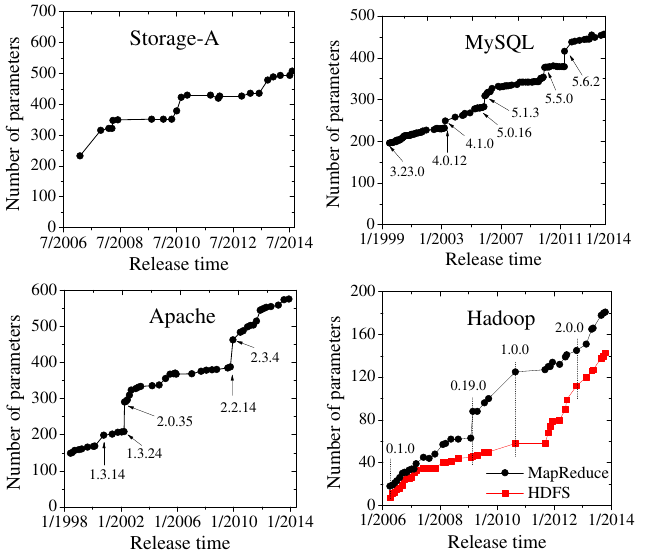
\includegraphics[scale=0.5]{pics/trend.png}
	\citet{xu2015hey}
\end{frame}

\subsection{Calculation}

\begin{frame}
	\frametitle{Types of Complexity}
	\begin{itemize}
	\item complexity in access:
		\begin{itemize}
		\item many different formats
		\item non-uniformity
		\item transformations
		\end{itemize}
	\item configuration settings
		\begin{itemize}
		\item number of settings $s$
		\item number of values $n$
		\item dependences between settings
		\end{itemize}
	\end{itemize}
\end{frame}

\lstDeleteShortInline^
\begin{frame}
	\frametitle{Calculation of Complexity}

	Using enumerative combinatorics:
	\begin{itemize}
	\item number of configurations: $n^s$
	\item for $N$ groups of different $n$ and $s$ (i.e., $n_1 \dots n_N$ with $s_1 \dots s_N$ occurrences):  $$\prod_{i=1}^{N} n_i^{s_i}$$
	\item more difficult to calculate (or unbounded) for dependences, module instantiations, arrays, \dots
	\end{itemize}
\end{frame}

\begin{frame}
	\frametitle{Calculation of Complexity}

	Examples:
	\begin{itemize}
	\item 600 boolean settings in Apache httpd (let us assume $n=2$):
	\pause
	$2^{600} \approx 10^{180}$

	\item 19 integer settings:
	\pause
	${2^{32}}^{19} = 2^{32 \cdot 19} = 2^{609} \approx 10^{183}$

	\item 2000 boolean settings in Firefox~\cite{jin2014configurations}:
	\pause
	$2^{2000} \approx 10^{602}$
	\end{itemize}
\end{frame}

%TODO: Firefox and LibreOffice is known, see calculation in jin2014configurations (RQ 1)

\begin{frame}
	\frametitle{Calculation of Complexity (cont.)}

	Examples:
	\begin{itemize}
	\item for 20 boolean and 20 enums with 5 possibilities:
	\pause
	$$2^{20}*5^{20} = 10^{20}$$

	\item MySQL has 461 settings, of which 216 are non-simple types~\cite{xu2015hey} \\ (let us assume $n=\{3,20\}$):
	\pause
	$3^{245} * 20^{216} \approx 10^{397}$ \\
	(settings are explained in 5560 pages\footnote{\url{https://downloads.mysql.com/docs/refman-5.7-en.pdf}})

	\item an array with $1-20$ boolean settings:
	\pause
	$2^{20}$
	\end{itemize}
\end{frame}
\lstMakeShortInline[postbreak=,keywordstyle={},showspaces=no]^
%XXX

\begin{assignment}
	\begin{task}
	Calculate complexity for some tool you know.
	\end{task}

	\begin{task}
	Possible Homework: Write tool to calculate complexity with a given configuration specification.
	\end{task}
\end{assignment}

\begin{frame}
	\frametitle{Decision Tree}
	\begin{itemize}
	\item configuration settings may depend on each other
	\item form a decision tree~\cite{reiser2009cvm,czarnecki2012cool}
	\item the decision tree is an instantiation of chosen configuration settings
	\item calculation only needs to consider instantiations which make a difference: \\
	essential configuration complexity~\cite{meinicke2016essential}
	\end{itemize}
\end{frame}

\subsection{Usage}

\begin{frame}[fragile]
	\frametitle{Harmful Defaults~\cite{xu2015hey}}
	\begin{itemize}
	\item Problem: Two major data losses on a dozen machines.
	\item Cause:
	Stayed with the default values of the data-path settings
	(e.g., ^dfs.name.dir^, ^dfs.data.dir^) which point to locations in ^/tmp^.
	Thus, after the machines reboot, data losses occur.
	``One of the common problems from users.'' (from Cloudera)
	\item up to \p{53} of misconfigurations is due to staying at defaults
	\item \p{17} to \p{48} of configuration issues are about difficulties in finding settings
	\end{itemize}
\end{frame}

\begin{frame}[fragile]
	\frametitle{Unnecessary Settings~\cite{xu2015hey}}
	\begin{itemize}
	\item Configuration Parameter: ^dfs.namenode.tolerate.heartbeat.multiplier^
	\item Developers' Discussion:
	Since we are not sure what is a good choice, how about making it
	configurable?
	We should add a configuration option for it. Even if it's unlikely to
	change, if someone does want to change it they'll thank us that they
	don't have to change the code/recompile to do so.
	\item Real-World Usage:
	\begin{itemize}
	\item No usage found by searching the entire mailing lists and Google.
	\item No usage reported in a survey of 15 Hadoop users in UCSD.
	\end{itemize}
	\end{itemize}
\end{frame}

\begin{frame}
	\frametitle{Unnecessary Settings~\cite{xu2015hey}}
	\begin{itemize}
	\item \p{6} to \p{17} of settings set by majority
	\item up to \p{54} are seldom set
	\item up to \p{47} of numeric settings have no more than five distinct values
	\end{itemize}
\end{frame}

\begin{frame}
	\frametitle{Reduction}
	\methodQuestion{}
	\question{Why do you think configuration should be reduced?}
	\begin{itemize}
	\item to simplify code maintenance (\p{50}),
	\item to prevent errors and misconfiguration (\p{43}),
	\item to provide better user experience (\p{40}),
	\item \textbf{\question{I do not think it should be reduced} (\p{30})},
	\item because they prefer auto-detection (\p{29}) \\ (with a possibility to override configuration settings: \p{32}),
	\item \question{because use-cases which are rarely used should not be supported} (\p{13}),
	\item \question{never find time for this task} (\p{9}), and
	\item \question{because only standard use-cases should be supported} (\p{1})
	\end{itemize}
\end{frame}

\begin{frame}
	\begin{alertblock}{Question}
	How to specify reduction strategies of configuration settings?
	\end{alertblock}
	\pause
	\begin{exampleblock}{Answer}
	Configuration Specification
	\end{exampleblock}
\end{frame}



%%%%%%%%%%%%%%%%%%%%%%%%%%%%%%%%%%%%%%%%%% 
\section{Configuration Specification}

\subsection{Why?}

\begin{frame}
	\frametitle{Rationale}
	\begin{itemize}
	\item without specification you and others do not even know which settings are available
	\item needed for any further techniques we will discuss
	\pause
	\item essential for \intro[no-futz computing]{no-futz computing}~\citet{holland2001nofutz}
	\item the foundation for any advanced tooling like configuration management tools
	\pause
	\item needed as communication of producers and consumers of configuration
	\end{itemize}
\end{frame}

\begin{assignment}
	\begin{task}
	Brainstorming: What can be part of a configuration specification?
	\end{task}

	\begin{task}
	Advantages/Disadvantages?
	\end{task}

	\begin{task}
	Alternatives?
	\end{task}
\end{assignment}

\begin{frame}
	\methodQuestion{}
	\question{Configuration specification (e.g. XSD/JSON schemas) allows you to describe possible values and their meaning.  Why do/would you specify configuration?}
	\ExecuteMetaData[../book/motivation.tex]{question-introduce-spec}
\end{frame}

\begin{frame}
	\frametitle{Limitations of Schemata designed for Data}
	\begin{itemize}
	\item like XSD/JSON schemas
	\item they are already very helpful but:
	\pause
	\item not key-value based
	\item not easy to introspect
	\item designed to validate data without semantics: \\ file path vs.\ presence of file
	\item not always possible to extend with plugins
	\item tied to specific formats (e.g. XML/JSON)
	\end{itemize}
\end{frame}

\begin{frame}
	\frametitle{Limitations of Zero-Configuration}
	\begin{itemize}
	\item e.g. gpsd\footnote{\url{www.aosabook.org/en/gpsd.html}}
	\pause
	\item broken hardware or protocols
	\item auto-detection may go wrong
	\item the configuration actually lives elsewhere \\ (e.g., in the GPS devices)
	\end{itemize}
\end{frame}

\subsection{How?}

\begin{frame}
	\frametitle{Types of Specifications}
	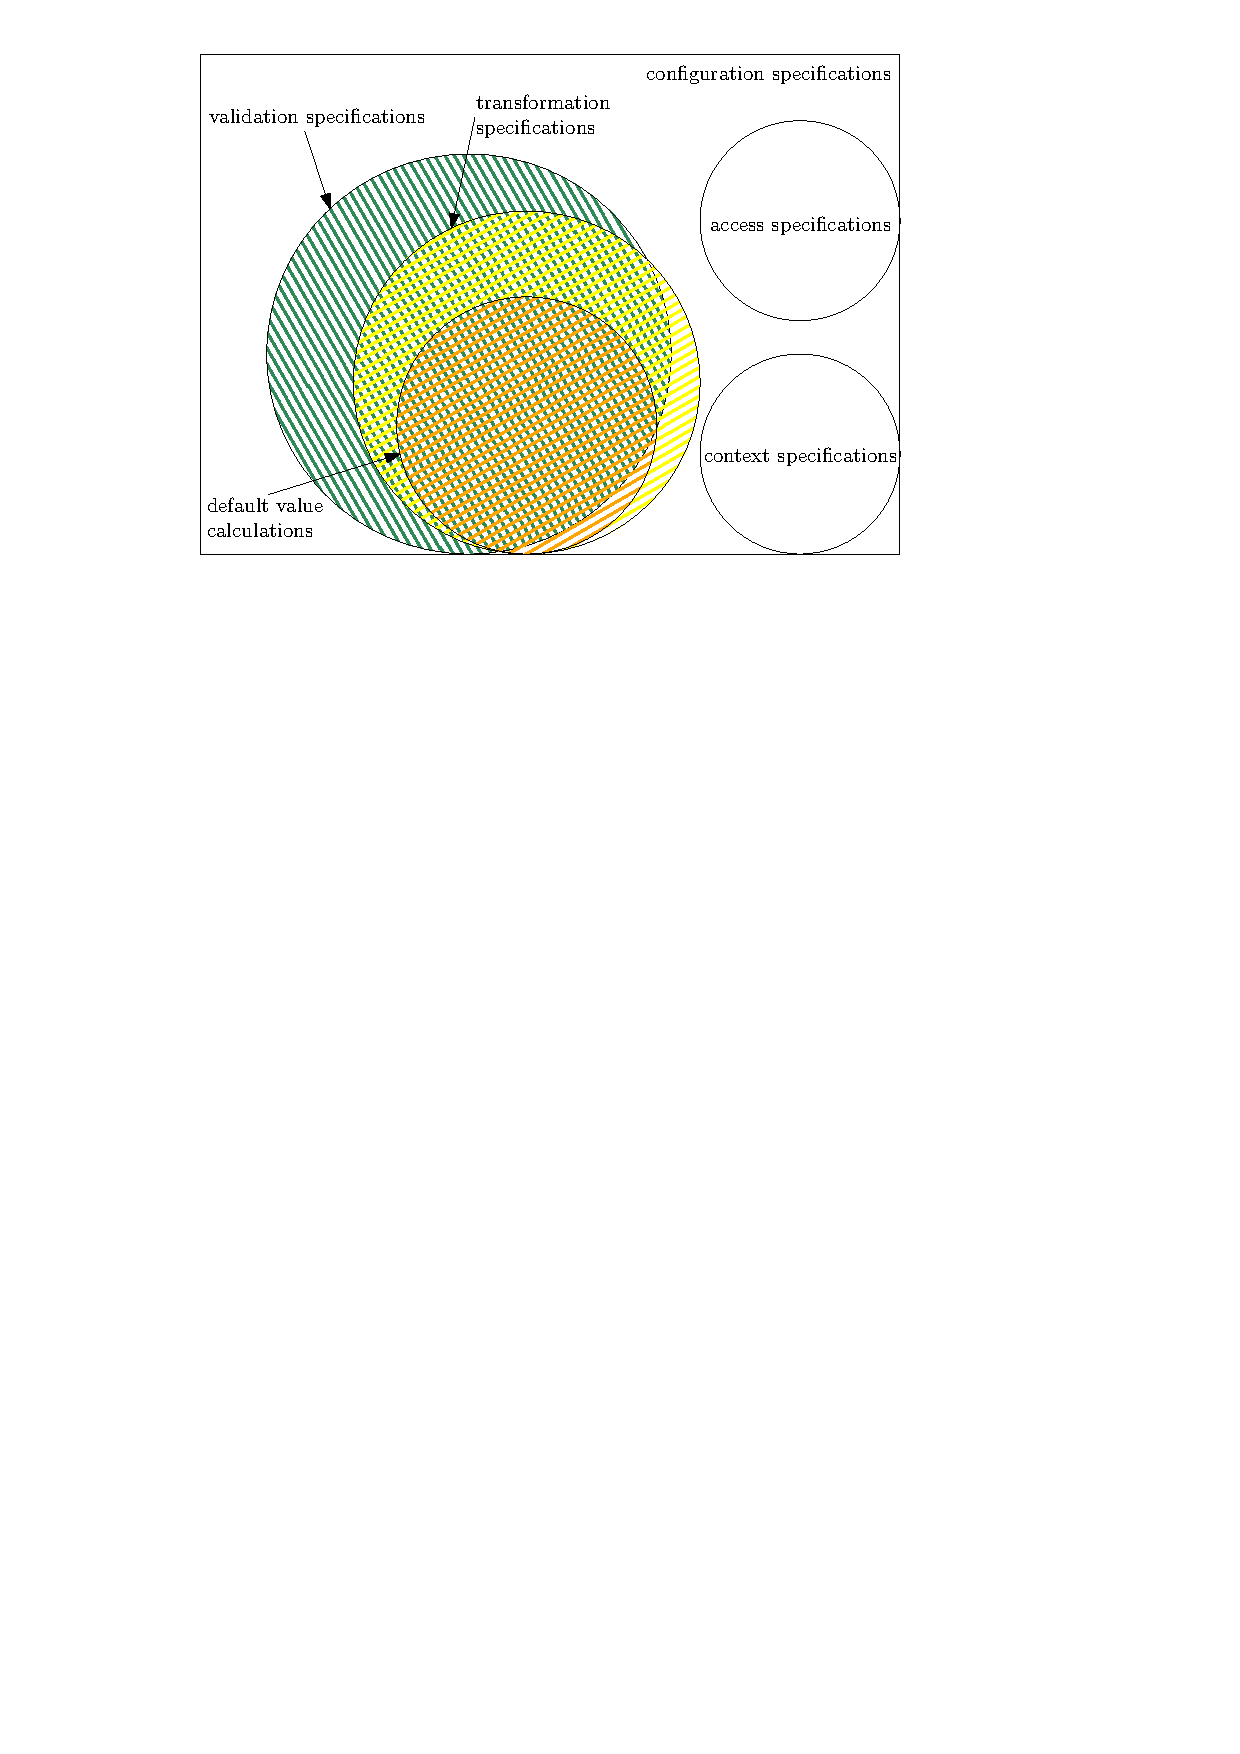
\includegraphics[scale=0.8]{specifications}
\end{frame}

\begin{frame}
	\frametitle{Metalevels}
	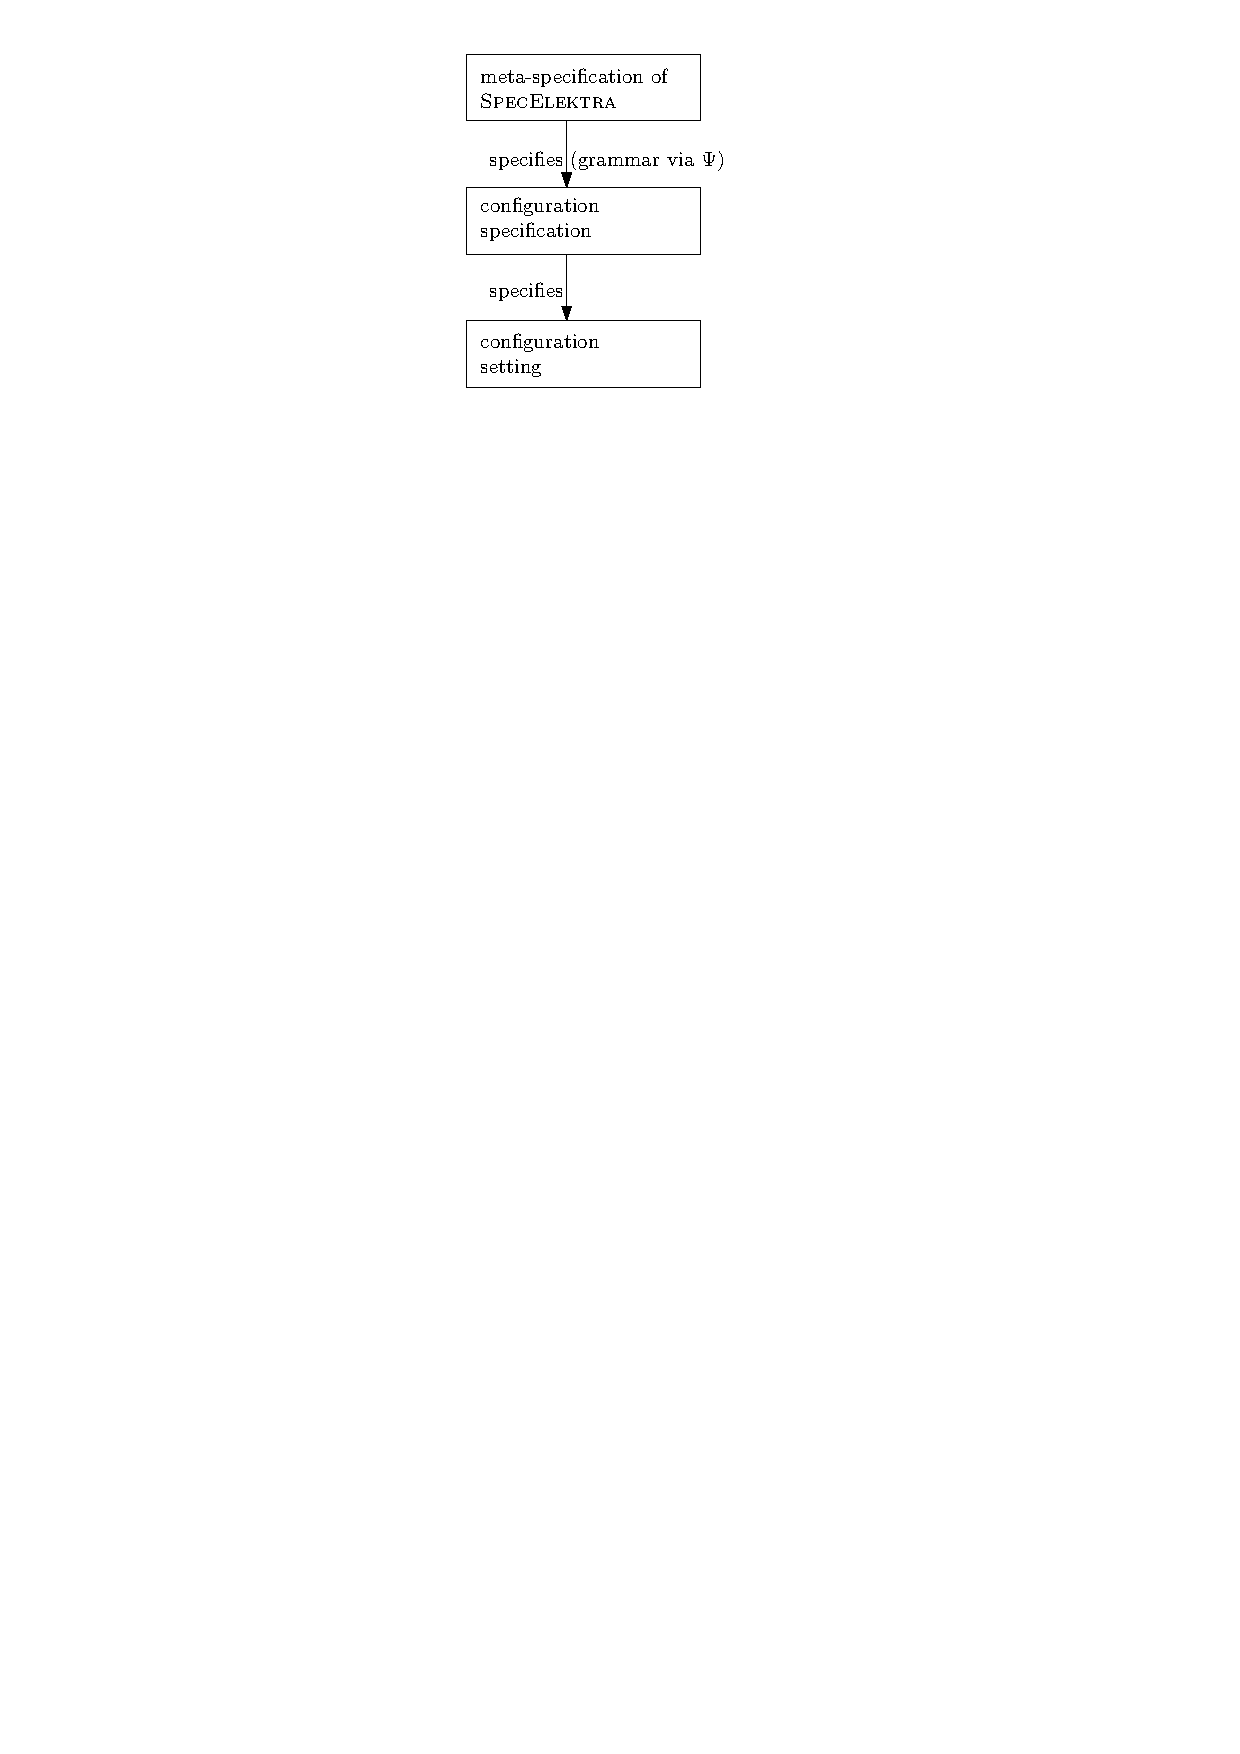
\includegraphics{metalevels}
\end{frame}

\begin{assignment}
	\begin{task}
	What do we mean with a configuration specification?
	\end{task}

	\begin{task}
	Which requirements do we have for a configuration specification?
	\end{task}
\end{assignment}


\begin{frame}
	\frametitle{Requirements}

	\begin{itemize}
	\item formal/informal?
	\item complete?
	\pause
	\item should be extensible
	\item should be external to application
	\item open for introspection (for tooling)
	\item should talk to users
	\item should allow generation of artefacts
	\end{itemize}
\end{frame}


\begin{frame}[fragile]
	\frametitle{Grammar}
	\begin{grammar}
	<configuration specifications> ::= \{ <configuration specification> \}

	<configuration specification> ::= '[' <key> ']' <properties>

	<properties> ::= \{ <property> \}

	<property> ::= <property name> ':=' [ <property value> ]
	\end{grammar}
\end{frame}


\begin{frame}[fragile]
	\frametitle{Example}
	\begin{code}[gobble=4]
	[slapd/threads/listener]
	default:=1
	type:=int
	\end{code}
\end{frame}

\subsection{Visibility}

\begin{frame}
	\frametitle{Visibility}
	\begin{itemize}
	\item idea: show only relevant settings for specific user group
	\item or disallow editing: accessibility
	\pause
	\item requires user-feedback loops~\cite{xu2015hey}
	\item most-used settings should be best visible (or even enforce them to be changed: against harmful defaults)
	\item think of your users (administrators), \\ only expose what users need
	\item write an rationale why someone needs it
	\end{itemize}
\end{frame}

\begin{frame}[fragile]
	\frametitle{Example}
	\begin{code}[gobble=4]
	[slapd/threads/listener]
	visibility:=developer

	[slapd/access/#]
	visibility:=user
	\end{code}
\end{frame}


\begin{assignment}
	\begin{task}
	Brainstorming: Now, how do we implement such a specification?
	\end{task}
\end{assignment}

\begin{frame}
	\frametitle{Implementations}
	For example:
	\begin{itemize}
	\item generate examples/documentation
	\item auto-completion/syntax highlighting/IDE support
	\item tooling (GUI, Web UI)
	\item validate configuration files
	\item visudo-like
	\item plugins in configuration framework
	\end{itemize}
\end{frame}

\subsection{Calculate Default Values}

\begin{frame}
	\begin{itemize}
	\item idea: make default value better
	\item is the generalization of sharing configuration values
	\item can be combined with visibility
	\pause
	\item can be derived from other configuration settings
	\item can be derived from context~\cite{raab2017introducing}
	\item can be derived from hardware/system (problem with dependences)
	\pause
	\item XServer vs.\ gpsd
	\end{itemize}
\end{frame}

\begin{frame}[fragile]
	\frametitle{Examples}
	Sharing:
	\begin{code}[gobble=4]
	[slapd/threads/listener]
	fallback/#0:=slapd/threads
	\end{code}

	\vspace{1cm}
	Percentages
	\\ (e.g., configured image should be additionally cropped):
	\pause
	\begin{code}[gobble=4]
	[image/width]
	type:=int

	[crop]
	type:=int
	check/range:=0-100
	\end{code}
\end{frame}

\begin{frame}[fragile]
	\frametitle{Examples}
	Context:
	\begin{code}[gobble=4]
	[slapd/threads/listener]
	context:=/slapd/threads/%cpu%/listener
	\end{code}

	\vspace{1cm}
	Calculation with Context
	\\ (e.g., switch off GPS if battery low):
	\pause
	\begin{code}[gobble=4]
	[gps/status]
	assign:=(battery > 'low') ? ('on') : ('off')
	\end{code}
\end{frame}



%%%%%%%%%%%%%%%%%%%%%%%%%%%%%%%%%%%%%%%%%% 
\section{Architectural Decisions}

\begin{frame}
	\frametitle{Software Architecture}
	\begin{itemize}
	\item architecture is high-level description of the overall system
	\item use ready-made patterns and templates for architecture
	\pause
	\item e.g., \url{http://arc42.org/}
	\item architectural decisions~\cite{zdun2007patterns} essential (e.g., Chapter~9 in arc42)
	\end{itemize}
\end{frame}

\begin{frame}
	\frametitle{Architectural Decisions}
	\begin{itemize}
	\item describe decisions that lead to the architecture
	\item open decisions are high-level configuration
	\item useful to have patterns~\cite{zdun2007patterns} and templates, too
	\item template: problem, constraints, assumptions, considered alternatives, decision, rationale, implications, related, notes
	\end{itemize}
\end{frame}

\begin{frame}
	Why are configuration settings added? \\[1cm]
	\pause
	The typical reasons are:
	\ExecuteMetaData[../book/implications.tex]{reasons-adding}
\end{frame}

\begin{frame}[fragile]
	\frametitle{in Configuration Specification}
	\begin{code}[gobble=4]
	[slapd/threads/listener]
	description:=adjust to use more threads
	rationale:=needed for many-core systems
	requirement:=1234
	visibility:=developer
	\end{code}
\end{frame}

\begin{frame}
	\frametitle{Conclusion}
	\begin{itemize}
	\item alarming trend in number and complexity of configuration settings
	\item sharing, visibility and default value calculation often helps
	\item needs abstraction: configuration specification
	\item but also more courageous decisions and periodical reevaluation
	\item different ways to reduce configuration space
	\end{itemize}
\end{frame}



%%%%%%%%%%%%%%%%%%%%%%%%%%%%%%%%%%%%%%%%%% 
\nocite{raab2017introducing}

\appendix

\begin{frame}[allowframebreaks]
	\bibliographystyle{plainnat}
	\bibliography{../shared/elektra.bib}
\end{frame}

\end{document}


